%!TEX root=main.tex
\section{应用}
\label{clicknp:sec:application}

为了评估 \name 的灵活性,我们基于 \name 创建了五个常见的NF。
所有这些都可以在我们的测试床处理实时流量中运行。
表 \ref {clicknp:tab:applications}总结了每个网络功能中包含的元素数量和总LoC,包括所有元素规范和配置文件。
我们的经验也证实了\name 的模块化架构极大地改善了代码重用并简化了新NF的构建。
如表 \ref {clicknp:tab:elements}所示,在许多应用程序中有很多机会重用一个元素,例如,本文(A1-5)中所有五个NF都使用了L4\_Parser。
每个NF可能需要1个左右的时间才能让一个程序员进行开发和调试。
我们发现联合CPU / FPGA处理的能力也将极大地帮助调试,因为我们可以将有问题的元素移动到CPU,以便我们可以轻松地打印日志来跟踪问题。

在下文中,我们将详细讨论这些NF。

\textbf {A1. 数据包生成器(PktGen)和捕获(PktCap)。}
PktGen可以根据不同的配置文件生成各种流量模式。
它可以生成不同大小的流,并根据给定的分布安排它们在不同的时间开始。
生成的流可以进一步通过不同的流量整形器来控制流速及其突发性。
PktCap只是将收到的所有数据包重定向到\textit {logger}元素,这些元素通常位于主机中。
由于单个记录器无法充分利用PCIe I / O通道容量,因此PktCap在FPGA中具有接收端缩放(RSS)元素,以根据流5元组的散列将数据包分发到多个记录器。
由于我们的PCIe通道的容量小于40G NIC,我们添加了一个\textit {extractor}元素,它只提取数据包的重要字段(例如,如果有5个元组,DSCP和VLAN标记),并转发这些字段(总共16B) ,以及跨PCIe的记录器元素的时间戳(4B)。
PktCap就是一个展示联合CPU / FPGA处理重要性的例子。
与FPGA相比,CPU具有更多的内存用于缓冲,并且可以轻松访问其他存储,例如,\cite{lee2015flosis}中的HDD / SSD驱动器,因此在CPU上运行记录器更有意义。


\textbf {A2. OpenFlow 防火墙(OFW)。}
我们的Openflow~\cite {mckeown2008openflow} 防火墙支持流的精确匹配和通配符匹配。
精确匹配表是使用Cuckoo Hashing \cite{cuckoo} 实现的,包含与流5元组匹配的128K条目。
模糊匹配匹配基于TCAM。
	但是,具有512个104位条目的简单TCAM实现占用了FPGA的65%逻辑资源。
	相反,我们使用基于BRAM的TCAM \cite {jiang2013scalable}。
	基于BRAM的TCAM将搜索密钥分解为8位密钥,并使用它们来寻址查找表,这些表将内存换成逻辑区域。具有2K条目的BRAM TCAM需要14%逻辑和43%的BRAM。
	此外,我们设计了一个HashTCAM来利用流表中的许多条目共享相同的位掩码这一事实。
	HashTCAM将表空间划分为许多较小的哈希表,每个哈希表都与一个位掩码相关联。
	在查找哈希表之前,任何传入的数据包都将首先执行“和”操作。
	表中的每个条目也与优先级相关联。
	仲裁器(multiplexer)选择具有最高优先级的匹配条目。
	HashTCAM在功能和区域成本之间有更好的权衡。
	具有16K流条目和16个不同位掩码的HashTCAM(类似于Broadcom Trident II~\cite {broadcomethernet})需要19%逻辑和22%BRAM。
	管理器程序总是尝试根据其位掩码对规则进行分组,并将具有大多数规则的组放入HashTCAM。
	然后将其余规则放入基于BRAM的TCAM中,这些规则不适合HashTCAM中的任何组。


\textbf{A3. IPSec网关(IPSecGW)。}
软件NF的一个问题是,当数据包需要一些计算密集型处理时,CPU很快就会成为瓶颈,例如,IPSec \cite {packetshader}。
我们构建了一个IPSec数据路径,能够使用AES-256-CTR加密和SHA-1身份验证处理IPSec数据包。
如\S \ref {clicknp:subsec:lib}所示,单个AES\_CTR元素只能实现27.8~Gbps的吞吐量。因此,我们需要两个AES\_CTR元素并行运行以实现线速率。
然而,SHA-1很棘手。 SHA-1将数据包分成较小的数据块(64B)。
虽然一个数据块中的计算可以流水线化,但是一个IP数据包内的连续块之间存在依赖关系 - 下一个块的计算无法在前一个块完成之前开始!
如果我们按顺序处理这些数据块,吞吐量将低至1.07 Gbps。
幸运的是,我们可以利用不同数据包之间的并行性。
虽然当前数据包的数据块的处理仍在进行,但我们提供了不同数据包的数据块。
由于这两个数据块没有依赖关系,因此可以并行处理它们。
为了实现这一点,我们设计了一个名为\textit {reservo}的新元素(保留站的简称),它可以缓冲多达64个数据包,并为SHA-1元素调度独立的块。在计算了一个数据包的签名之后,\textit {reservo}元素将它发送到将SHA-1 HMAC附加到数据包的下一个元素。
还有一件棘手的事情。
虽然SHA-1元素具有固定的延迟,但数据包的总延迟是不同的,即与数据包大小成比例。
当在SHA-1计算中调度多个分组时,这些分组可能是无序的,例如,大分组后面的较小分组可能更早地完成。
为了防止这种情况,我们在SHA-1元素之后进一步设计了一个\textit {reorder buffer}元素,该元素存储无序数据包并根据数据包的序列号恢复原始顺序。

\textbf {A4. L4负载平衡器(L4LB)。}
我们根据Ananta~ \cite {ananta}中的\textit {multiplexer}(MUX)实现L4LB。
MUX服务器基本上查看数据包标头,并查看是否已为该流分配了\textit {直接地址}(DIP)。
如果是,则通过NVGRE隧道将分组转发到由DIP指示的服务器。否则,MUX服务器将调用本地控制器为流分配DIP。
MUX服务器中需要按流状态。
由于存在故障并且避免黑洞需要即时更改后端服务器列表,因此无法使用基于散列的ECMP。此外,高级LB还可能需要负载感知平衡。
流表用于记录流向其DIP的映射。
为了处理数据中心的大流量,它需要L4LB在流表中支持多达3200万个流。
显然,如此大的流量表不能适应FPGA的BRAM,必须存储在板载DDR存储器中。
但是,访问DDR内存很慢。
为了提高性能,我们在BRAM中创建了一个带有16K高速缓存行的4路关联流缓存。最近最少使用(LRU)算法用于替换流缓存中的条目。

在我们的实现中,传入的数据包首先传递一个\textit {解析器}(parser)元素,该元素提取5元组并将它们发送到\textit {流缓存}(flow cache)元素。
如果在流缓存中找不到流,则将数据包的元数据转发到全局流表,该表读取DDR中的完整表。
如果仍然没有匹配的条目,则该数据包是流的第一个数据包,并且请求被发送到\textit {DIPAlloc}元素,以根据负载平衡策略为该流分配DIP。
确定DIP后,将一个条目插入到流表中。

在确定分组的DIP之后,封装元件将检索下一跳信息,例如IP地址和VNET ID,并相应地生成NVGRE封装的分组。
对于流的剩余分组,从流状态提取DIP。
如果收到FIN数据包或发生超时,则流条目将无效
在从流中接收任何新数据包之前。
在确定DIP之后,我们从BRAM检索下一跳元数据并封装NVGRE头以将分组引导到分配的DIP。

除了\textit {DIPAlloc}元素之外,我们将所有元素都放在FPGA中。
由于只有流的第一个数据包可能会出现\textit {DIPAlloc}并且分配策略也可能很复杂,因此更适合运行
CPU上的\textit {DIPAlloc},是联合CPU-FPGA处理的另一个例子。

%
\egg{
To handle the large traffic volume in datacenters, it requires the L4LB to support up to 32 million flows in the flow table.
Clearly, such a large flow table cannot fit into the BRAM of FPGA, and has to be stored in onboard DDR memory.
Accessing DDR memory is slow. To improve performance, we further create a 4-way associative flow cache in BRAM with 16K 
cache lines. The flow cache is replaced based on the Least Recently Used (LRU) algorithm.
DDR memory access is a fat pipeline stage as shown in Figure \ref{clicknp:fig:unbalance}. We move the DDR access part to a separate element to make the fast path run asynchronously with slow path.}



\textbf {A5. pFabric 流调度程序。}
我们使用\name 来实现一个最近提出的数据包调度规则--pFabric \cite {pfabric}。
pFabric调度很简单。它只保留浅缓冲区(32个数据包),并始终使具有最高优先级的数据包出列。当缓冲区已满时,优先级最低的数据包将被丢弃。
pFabric显示在数据中心中实现接近最佳的流完成时间。
在原始论文中,作者提出使用二进制比较树(Binary Comparison Tree,BCT)来选择具有最高优先级的数据包。
但是,虽然BCT只需要$O(log_2 N)$个周期来计算最高优先级的数据包,但在连续的选择过程之间存在依赖关系。这是因为只有当前一个选择完成后我们才能知道最高优先级的数据包,然后才能可靠地启动下一个选择过程。
这种限制要求时钟频率至少为300MHz才能实现40Gbps的线速,这对我们当前的FPGA平台来说是不可能的。
在本文中,我们使用不同的方式来实现pFabric调度程序,它更容易并行化。
该方案基于\textit{移位寄存器优先级队列}(shift register priority queue) \cite {moon2000scalable}。
条目以非增加优先级顺序保存在$K$个寄存器中。
出列时,所有条目都向右移动并弹出头部。这只需要1个周期。
对于入队操作,新数据包的元数据将转发到所有条目。
现在,对于每个条目,可以在条目中的分组,新分组和相邻条目中的分组之间执行本地比较。
由于所有局部比较都可以并行进行,因此入队操作也可以在1个周期内完成。
入队和出队操作可以进一步并行化。
因此,可以在一个周期中处理分组。

\textbf{A6. 容错的 LTE SPGW。}

\textbf{A7. 端口扫描检测。}

\textbf{A8. HTTPS RSA 加速。}

\textbf{A9. 正则表达式匹配。}

\textbf{A10. 神经网络推理。}

\egg{
pFabric \cite{alizadeh2013pfabric} is a near-optimal datacenter transport based on priority scheduling and dropping. Packets are scheduled based on its flow size or remaining flow size in a small queue. Our pFabric scheduler implementation (Figure \ref{clicknp:fig:PFabric}) support 4-giga strict priorities, including a PriorityQueue which deques the packet with highest priority and drops overflow packets with lowest priority, a ReorderQueue to find the earliest packet from the flow with highest priority to avoid starvation and keep packet ordering, and a PacketBuffer to receive packets into buffer and schedule or drop packets out of buffer. Since queue size in a perfectly load balanced fabric should be small, we choose shift register priority queue for maximum throughput and clock frequency.

ReorderQueue is another shift register queue ordered by flow hash. On enque command from PacketBuffer, packet metadata with flow hash $f_{new}$ is enqued to entry $i$ where $f_{i-1} < f_{new} \leq f_{i}$. On deque command from PriorityQueue, the entry $i$ with $f_{i} = f_{deque} < f_{i+1}$ is dequed. Packets with a same flow hash are dequed in the same order as they are enqued.


\begin{figure}[h!]
	\centering
	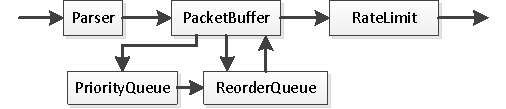
\includegraphics[width=1.0\columnwidth]{image/PFabric}
	\vspace{-0.30in}
	\caption{PFabric Element Graph}
	\vspace{-0.10in}
	\label{clicknp:fig:PFabric}
	%    
\end{figure}
}
